\documentclass[12pt,english,a4paper]{article}
\pdfobjcompresslevel=0
\usepackage[usenames,dvipsnames]{xcolor}
\usepackage[includeheadfoot,margin=0.8 in,top=0.6 in]{geometry}
\usepackage{siunitx,physics,cancel,upgreek,varioref,listings,booktabs,tocloft, pdfpages}
\usepackage{todonotes}
\usepackage{mathtools}
\usepackage{babel}
\usepackage{graphicx}
\usepackage{float}
\usepackage{fouriernc}
\usepackage{fancyhdr}
\usepackage[utf8]{inputenc}
\usepackage{amsmath}
\usepackage{amssymb}
\usepackage{textcomp}
\usepackage{lastpage}
\usepackage{microtype}
\usepackage{ifthen}
\usepackage{longtable}
\usepackage[linktoc=all, bookmarks=true, pdfauthor={Anders Johansson}]{hyperref}
\renewcommand{\CancelColor}{\color{red}}
\renewcommand{\exp}[1]{\mathrm{e}^{#1}}
\newcommand{\R}{\mathbb{R}}
\newcommand{\tittel}[1]{\title{#1 \vspace{-7ex}}\author{}\date{}\maketitle\thispagestyle{fancy}\pagestyle{fancy}\setcounter{page}{1}}

\newcommand{\deloppg}[2][]{\subsection*{#2) #1}\addcontentsline{toc}{subsection}{#2)}\refstepcounter{subsection}\label{#2}}
\newcommand{\oppg}[1]{\section*{Oppgave #1}\addcontentsline{toc}{section}{Oppgave #1}\refstepcounter{section}\label{oppg#1}}

\labelformat{section}{section~#1}
\labelformat{subsection}{section~#1}
\labelformat{subsubsection}{section~#1}
\labelformat{equation}{equation~(#1)}
\labelformat{figure}{figure~#1}
\labelformat{table}{table~#1}

\lstset{rangeprefix=/*\#,
rangesuffix=\#*/,
includerangemarker=false}
\renewcommand{\lstlistingname}{Code snippet}
\definecolor{codegreen}{rgb}{0,0.6,0}
\definecolor{codegray}{rgb}{0.5,0.5,0.5}
\definecolor{codepurple}{rgb}{0.58,0,0.82}
\definecolor{backcolour}{rgb}{0.95,0.95,0.92}
\lstset{showstringspaces=false,
basicstyle=\footnotesize\ttfamily,
keywordstyle=\color{codegreen},
commentstyle=\color{magenta},
numberstyle=\tiny\color{codegray},
stringstyle=\color{codepurple},
frameshape={RYRYNYYYY}{yny}{yny}{RYRYNYYYY},
breaklines=true,
%literate={0}{{\textcolor{blue}{0}}}{1}%
%             {1}{{\textcolor{blue}{1}}}{1}%
%             {2}{{\textcolor{blue}{2}}}{1}%
%             {3}{{\textcolor{blue}{3}}}{1}%
%             {4}{{\textcolor{blue}{4}}}{1}%
%             {5}{{\textcolor{blue}{5}}}{1}%
%             {6}{{\textcolor{blue}{6}}}{1}%
%             {7}{{\textcolor{blue}{7}}}{1}%
%             {8}{{\textcolor{blue}{8}}}{1}%
%             {9}{{\textcolor{blue}{9}}}{1}%
%             {.0}{{\textcolor{blue}{.0}}}{2}% Following is to ensure that only periods
%             {.1}{{\textcolor{blue}{.1}}}{2}% followed by a digit are changed.
%             {.2}{{\textcolor{blue}{.2}}}{2}%
%             {.3}{{\textcolor{blue}{.3}}}{2}%
%             {.4}{{\textcolor{blue}{.4}}}{2}%
%             {.5}{{\textcolor{blue}{.5}}}{2}%
%             {.6}{{\textcolor{blue}{.6}}}{2}%
%             {.7}{{\textcolor{blue}{.7}}}{2}%
%             {.8}{{\textcolor{blue}{.8}}}{2}%
%             {.9}{{\textcolor{blue}{.9}}}{2}%
}

\renewcommand{\footrulewidth}{\headrulewidth}
\tocloftpagestyle{fancy}

\setcounter{secnumdepth}{4}
\renewcommand{\thesection}{\arabic{section}}
\renewcommand{\thesubsection}{\arabic{section}.\arabic{subsection}}
\renewcommand{\thesubsubsection}{\arabic{section}.\arabic{subsection}.\arabic{subsubsection}}
\setlength{\parindent}{0cm}
\setlength{\parskip}{1em}

\newcommand{\eqtag}[1]{\refstepcounter{equation}\tag{\theequation}\label{#1}}
\hypersetup{colorlinks=true,urlcolor=blue,linkcolor=black}

\sisetup{detect-all}
\sisetup{exponent-product = \cdot, output-product = \cdot,per-mode=symbol}
\sisetup{output-decimal-marker={.}}
\sisetup{round-mode = off, round-precision=3}
\sisetup{number-unit-product = \ }
\DeclareSIUnit\year{yr}

\allowdisplaybreaks[4]
\fancyhf{}

\rhead{Kristine B. Hein and Anders Johansson}
\rfoot{Page \thepage{} of \pageref{LastPage}}
\lhead{FYS3150}
%
\usepackage[backend=biber,citestyle=numeric-comp,bibstyle=numeric,sorting=none]{biblatex}
\DefineBibliographyStrings{norsk}{%
  bibliography = {Referanser},
}
\DefineBibliographyStrings{english}{%
  bibliography = {References},
}
\addbibresource{kilder.bib}

\newcommand{\program}[1]{\href{https://github.com/anjohan/Project5/blob/master/#1}{#1}}


\title{FYS3150 Project 4}
\author{Kristine Baluka Hein and Anders Johansson}
\begin{document}
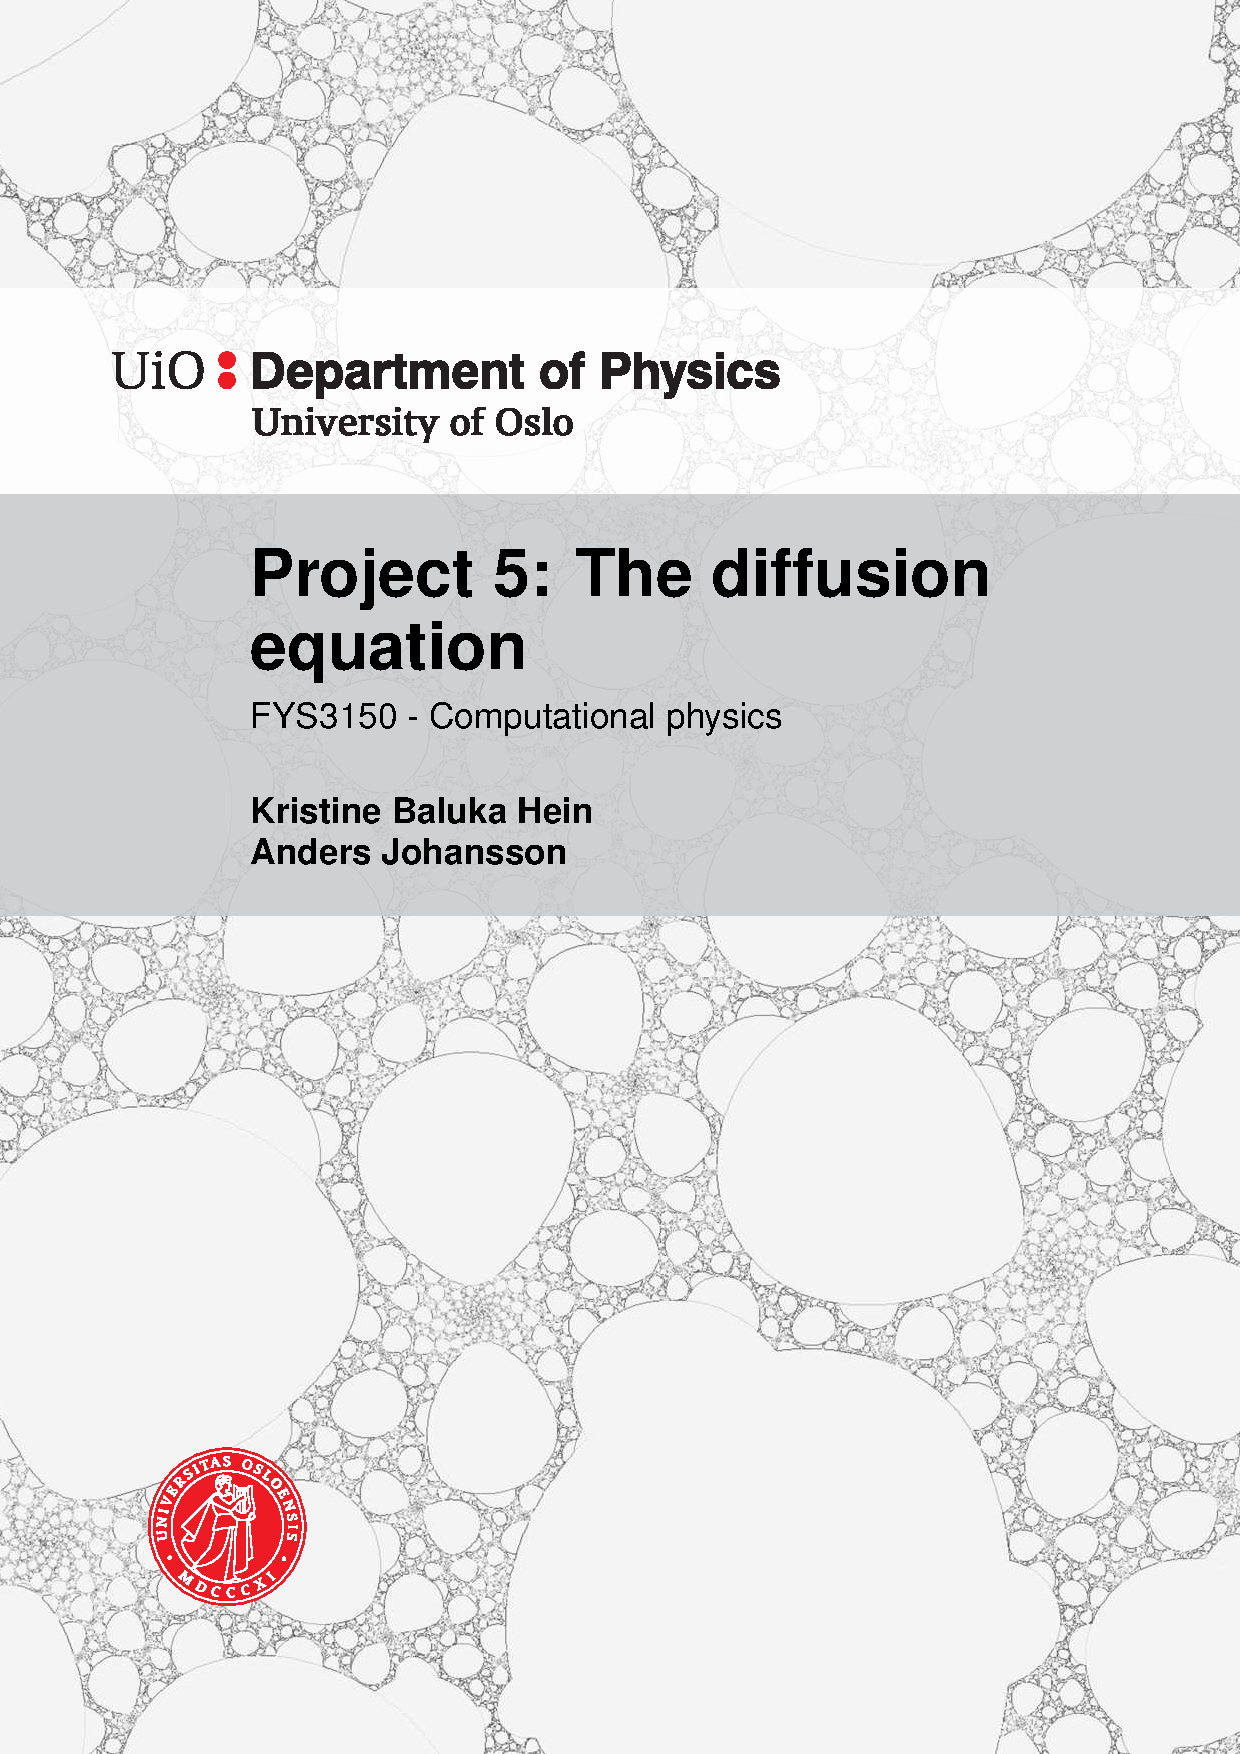
\includepdf{forside.pdf}
%\maketitle
\pagestyle{fancy}
\tableofcontents

\begin{abstract}
Hei.
\end{abstract}
\listoftodos
\clearpage

\section{Introduction}
Partial differential equations is a subject of many fields. These equations can describe the behavior of many natural phenomenas such as waves of sound or sea, the flow of a liquid, growth of a population or diffusion of different processes.

These equations are often solved numerically since an analytical solution is difficult, or perhaps impossible to find. An example is the Navier-Stokes equation to model the flow of a viscous flow when not certain assumptions to simplify the equations has been made.
\todo[inline]{skrive noe kult om diffusjon?}
In this report we will focus on how we can numerically solve the diffusion equation, which is given by
\begin{equation}\label{eq:diffusion}
\begin{aligned}
\pdv[2]{u(x,t)}{x} &= \pdv{u(x,t)}{t} &\: t>0, \:\:x\in[0,L] \\
u(x,0) &= 0  &0 < x < L\\
u(0,t) &= 0 &t>0 \\
u(L,t) &= 1&t>0
\end{aligned}
\end{equation}
with \(L = 1\).
\todo[inline]{noen fysiske forklaringer paa boundaries}


%   __           _ _    _
%  / _|_   _ ___(_) | _| | __
% | |_| | | / __| | |/ / |/ /
% |  _| |_| \__ \ |   <|   <
% |_|  \__, |___/_|_|\_\_|\_\
%      |___/
\section{Physical theory of diffusion}
Diffusion is simply the net movement of particles as a result of a random walk, and can be modelled as each atom constantly making a jump in a random  direction. It may seem a little counterintuitive that random motion can lead to a net flow, but consider that if there are \(10\) particles to the left, of which half move to the right, and \(100\) particles on the right, of which half move to the left, the net result is \(45\) particles moving to the left. The opposite of diffusion is drift, where the net motion is a result of an external driving force, for example an electric field.

The two most important equations in diffusion are Fick's laws, which, in one dimension, state that
\[
J = -D\pdv{C}{x} \qquad \qquad \pdv{C}{t} = D\pdv[2]{C}{x}
\]
where \(D\) is the diffusion coefficient, \(J\) the flux, i.e. the number of particles moving per area, and \(C\) the concentration, i.e. the number of particles per volume. Observe that Fick's second law, which is also simply called the diffusion equation, is the partial differential equation which is solved numerically on a dimensionless form in this project.

\subsection{Derivation of Fick's first law in one dimension}
\begin{figure}[H]
    \centering
    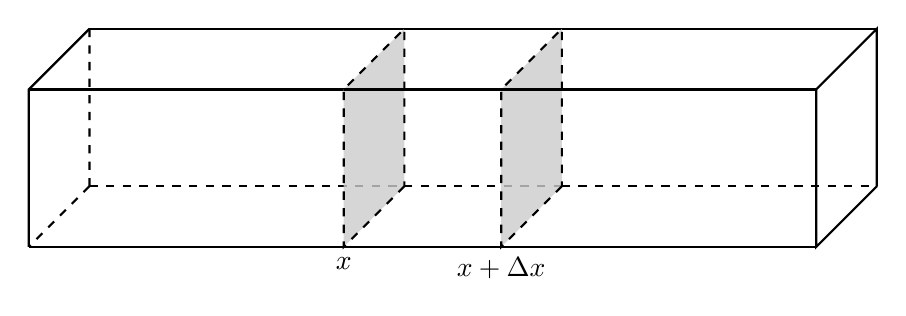
\begin{tikzpicture}[thick]
        \draw (0,0,2) -- (0,2,2) -- (0,2,0);
        \draw[dashed] (0,0,0) -- (0,0,2) (0,2,0) -- (0,0,0);
        \draw[dashed] (0,0,0) -- (4,0,0);
        \draw (0,0,2) -- (4,0,2);
        \draw (0,2,2) -- (4,2,2);
        \draw (0,2,0) -- (4,2,0);
        \fill[black!20!white,opacity=0.8] (4,0,0) -- (4,0,2) node[anchor=north] {\(x\)} -- (4,2,2) -- (4,2,0) -- (4,0,0);
        \draw[dashed] (4,0,0) -- (4,0,2) node[anchor=north] {\(x\)} -- (4,2,2) -- (4,2,0) -- (4,0,0);
        \draw[dashed] (6,0,0) -- (4,0,0);
        \draw (6,0,2) -- (4,0,2);
        \draw (6,2,2) -- (4,2,2);
        \draw (6,2,0) -- (4,2,0);
        \fill[black!20!white,opacity=0.8] (6,0,0) -- (6,0,2) -- (6,2,2) -- (6,2,0) -- (6,0,0);

        \draw[dashed] (6,0,0) -- (6,0,2) node[anchor=north] {\(x+\Delta x\)} -- (6,2,2) -- (6,2,0) -- (6,0,0);
        \draw[dashed] (6,0,0) -- (10,0,0);
        \draw (6,0,2) -- (10,0,2);
        \draw (6,2,2) -- (10,2,2);
        \draw (6,2,0) -- (10,2,0);
        \draw (10,0,0) -- (10,0,2) -- (10,2,2) -- (10,2,0) -- (10,0,0);
    \end{tikzpicture}
    \caption{Sketch of the infinitesimal volume element used the derivation of Fick's laws in one dimension.}\label{fig:fick}
\end{figure}

As stated above, diffusion is the process of random walk. In one dimension, this means that each particle will have a \(\SI{50}{\percent}\) probability of moving one step to the left, and a \(\SI{50}{\percent}\) probability of moving one step to the right. As such, the net movement of particles to the right between \(x\) and \(x+\Delta x\) equals half the particles at point \(x\) minus half the particles at point \(x+\Delta x\). Since the flux is the movement of particles per cross-section area \(A\) (marked with grey in the figure) per time interval \(\Delta t\), this can be formulated mathematically as
\[
    J = -\frac{N(x+\Delta x, t) - N(x,t)}{2A\Delta t}
\]
Multiplying by \(\qty(\Delta x)^2\) in both the numerator and the denominator, and factoring out the \(\Delta t\), we get
\[
    J = -\frac{\qty(\Delta x)^2}{2\Delta t}\qty(\frac{N(x+\Delta x,t) - N(x,t)}{A\Delta x\cdot\Delta x})
\]
Since \(A\Delta x\) is a small volume element, \(C=N/\qty(A\Delta x)\):
\[
    J = -\frac{\qty(\Delta x)^2}{2\Delta t} \qty(\frac{C(x+\Delta x,t) - C(x,t)}{\Delta x})
\]
Defining \(D=\qty(\Delta x)^2/2\Delta t\) and letting \(\Delta x\to0\) gives Fick's first law:
\[
    J = -D\pdv{C}{x}
\]

\subsection{Derivation of Fick's second law in one dimension}
The derivation of Fick's second law is based on finding two different expressions for the change in the number of particles between \(x\) and \(x+\Delta x\), setting them equal to each other and inserting Fick's first law into the result.

To find the change in number of particles between the two grey surfaces in \vref{fig:fick} over a time interval \(\Delta t\), remember that the flux is defined as the number of particles passing per cross-section \(A\) per time interval \(\Delta t\). Therefore, the number of particles moving out of the volume between \(x\) and \(x+\Delta x\) in a time interval \(\Delta t\) is \(J(x+\Delta x,t)A\Delta t\), while the number of particles moving into the volume is \(J(x,t)A\Delta t\). Thus, the net change in the number of particles between \(x\) and \(\Delta x\) can be written as
\[
    \qty(J(x,t) - J(x + \Delta x,t))A\Delta t = -\qty(J(x+\Delta x,t) - J(x,t))A\Delta t
\]
On the other hand, this change in the number of particles must also equal the change in concentration \(C(x,t+\Delta t) - C(x,t)\), multiplied with the volume, \(A\Delta x\). Since these two methods of calculating the change in the number of particles must give the same result, the following equation must hold:
\begin{alignat*}{2}
    -\qty(J(x+\Delta x,t) - J(x,t))A\Delta t &= \qty(C(x,t+\Delta t) - C(x,t)) A\Delta x\\
    \frac{J(x+\Delta x,t) - J(x,t)}{\Delta x} &= -\frac{C(x,t+\Delta t) - C(x,t)}{\Delta t}
\end{alignat*}
Letting \(\Delta x\to0\) and \(\Delta t\to0\), we get the so-called continuity equation:
\[
    \pdv{J}{x} = -\pdv{C}{t}
\]
Inserting Fick's first law for \(J\) on the left hand side, Fick's second law appears:
\begin{alignat*}{2}
    \pdv{x}\qty(-D\pdv{C}{x}) &= -\pdv{C}{t}\\
    D\pdv[2]{C}{x} &= \pdv{C}{t}
\end{alignat*}


\section{Mathematical theory}
Before we can begin our analysis on how it is possible to numerically solve \vref{eq:diffusion}, we will first take a look at the analytical solution. When having an analytical solution at hand, we can use it further to find which conditions the numerical methods must hold to give us stable results.
\subsection{Analytical solution of the diffusion equation}
Consider the diffusion equation with the given boundaries:
\begin{equation}\label{eq:problem}
\begin{aligned}
\pdv[2]{U(x,t)}{x} &= \pdv{U(x,t)}{t} &\: t>0, \:\:x\in[0,L] \\
U(x,0) &= g(x)  &0 < x < L\\
U(0,t) &=  a & a \in \mathbb{R},  t>0 \\
U(L,t) &= b &b \in \mathbb{R}, t>0
\end{aligned}
\end{equation}
First, we notice the boundaries at \(x = 0\) and \(x = L\). As we will see, having these boundaries equal to 0 would make the problem much easier to solve. Therefore, we introduce a new function
\[
v(x,t) = U(x,t) + w(x,t)
\]
where we want the following to hold:
\begin{equation}\label{eq:dummy}
\begin{aligned}
\pdv[2]{v(x,t)}{x} &= \pdv{v(x,t)}{t} &\: t>0, \:\:x\in[0,L] \\
v(x,0) &= f(x)  &0 < x < L\\
v(0,t) &=  0 &  t>0 \\
v(L,t) &= 0 & t>0
\end{aligned}
\end{equation}
By introducing \(v(x,t)\), we have also introduced a new problem; what does \(w(x,t)\) actually look like? We note that
\begin{alignat*}{2}
\pdv[2]{v(x,t)}{x} &= \pdv{v(x,t)}{t}  \\
\implies \pdv[2]{U(x,t)}{x} + \pdv[2]{w(x,t)}{x} &= \pdv{U(x,t)}{t} + \pdv{w(x,t)}{t}
\end{alignat*}
From \ref{eq:problem} we have that
\[
\pdv[2]{U(x,t)}{x} = \pdv{U(x,t)}{t}
\]
This means that if we set
\begin{equation} \label{eq:dummy1}
 \pdv[2]{w(x,t)}{x}  = 0
\end{equation}
and
\begin{equation} \label{eq:dummy2}
 \pdv{w(x,t)}{t} = 0
\end{equation}
the first condition for \(v(x,t)\) in \vref{eq:dummy} will hold. We can now find a general solution for \(w\). From \vref{eq:dummy1}, we have that
\begin{align}
	\pdv[2]{w(x,t)}{x}  &= 0 \nonumber \\
	\implies\pdv{w(x,t)}{x} &= A  \quad A \in \mathbb{R} \nonumber \\
	\implies w(x,t) &= Ax + B + h_1(t) \quad B \in \mathbb{R} \label{eq:wX}
\end{align}
From \vref{eq:dummy2}, we get that
\begin{align}
\pdv{w(x,t)}{t} &= 0 \nonumber \\
w(x,t) &= C + h_2(x) , \quad C \in \mathbb{R} \label{eq:wT}
\end{align}
From \vref{eq:wX} and \vref{eq:wT}, we see that
\[
w(x,t) = w(x) = Ax + D, \quad D=B+C
\]
because there is no dependence of \(t\) in \vref{eq:wT}.
We have now found how \(w\) looks like in general. \\
However, we need to decide the values of \(A\) and \(D\). This can be done by looking at the boundaries for \vref{eq:dummy} at \(x = 0 \) and \(x = L\):
\begin{align*}
v(0,t) &= 0 \\
0 &= U(0,t) + w(x=0) \\
0 &= a+D
\end{align*}
which implies \(D = -a\). Same goes for the boundary at \(x = L\), which gives
\begin{align*}
v(L,t) &= 0 \\
0 &= U(L,t) + w(x=L) \\
0 &= b+AL-a \\
\frac{a-b}{L} &= A
\end{align*}
In conclusion, we have
\[
w(x) = \frac{a-b}{L}x - a
\]
As the expression of \(w\) has been found, we have also found \(f(x)\) in \vref{eq:dummy}:
\begin{align*}
	v(x,0) &= U(x,0) + w(x) \\
	&= g(x)+w(x) \\
	&=f(x)
\end{align*}
Having set up the problem properly, we are now ready to solve for \(v(x,t)\). To do so, we make an ansatz that
\[
v(x,t) = F(x)G(t)
\]
which gives
\begin{align}
\pdv[2]{v(x,t)}{x} &= \pdv{v(x,t)}{t} \nonumber \\
F''(x)G(t) &= F(x)G'(t) \nonumber \\
\frac{F''(x)}{F(x)} &= \frac{G'(t)}{G(t)} \label{eq:ration}
\end{align}
Since the ratios of functions of different variables equals each other, they must be equal to a constant, thus giving
\[
\frac{F''(x)}{F(x)} = \frac{G'(t)}{G(t)} = -\lambda
\]
Solving for \(F\) we get
\[
	F'' = -\lambda F
\]
with a general solution
\[
F(x) = c_1\cos(x\sqrt{\lambda} ) + c_2\sin(x\sqrt{\lambda})
\]
To find the constants \(c_1,c_2\), we will use the boundaries for \(v(x,t)\) at \(x = 0\) and \(x = L\). At this point we will see that it is advantageous for us to have the boundaries equal to zero.\\
Since
\[
v(x,t) = F(x)G(t)
\]
We have
\[
0 = F(0)G(t) \implies F(0) = 0
\]
and
\[
0 = F(L)G(t) \implies F(L) = 0
\]
At \(x = 0\), the general solution becomes
\[
0 = c_1
\]
and at \(x = L\):
\[
0 =  c_2\sin(L\sqrt{\lambda})
\]
Of course, we could set \(c_2 = 0\) too, but this will only give us a trivial solution which is of no interest. Therefore, we must have
\[
0 = \sin(L\sqrt{\lambda})
\]
Since sine is zero for every multiple of \(\pi\), we have that
\begin{align*}
L\sqrt{\lambda} &= k\pi \quad k\in \mathbb{N}\\
\lambda &= \qty(\frac{k \pi}{L})^2
\end{align*}
We notice that we have infinite solutions since \(k \in \mathbb{N}\). Therefore, we might have a different scaling of sine for every \(k\), meaning \(c_2 = c_k\).\\  For every \(k\) we have the particular solution
\[
F_k(x) = c_k\sin(x\frac{k \pi}{L})
\]
Similar calculations goes for finding \(G(t)\), which also will vary with \(k\):\\
From \vref{eq:ration} we have
\[
G_k'(t) = -\lambda_k G_k(t)
\]
this gives
\[
G_k(t) = Ce^{-\qty(\frac{k \pi}{L})^2t}
\]
Since \(C\) is arbitrary, we could for simplicity set \( C = 1\). The contribution of \(C\) will anyway be indirectly a part of  \(c_k\). 
So, we have found the \(k\)th particular solution of \(G(t)\). \\
Therefore, we have that
\[
v_k(x,t) = c_ke^{-\qty(\frac{k \pi}{L})^2t}\sin(x\frac{k \pi}{L})
\]
What remains now is to find \(c_k\). We have not yet taken into account the boundary of \(v(x,t)\) when \(t = 0\). At \(t = 0\), we have that
\[
f(x) = c_k\sin(x\frac{k \pi}{L})
\]
Multiplying  the equation above by \(\sin(x\frac{k \pi}{L})\), integrating both sides and use the orthogonality of sine (note that this sine is \(L\)-periodic), gives us
\begin{align*}
\int_0^Lf(x)\sin(x\frac{k \pi}{L})dx &= c_k\frac{L}{2} \\
\frac{2}{L}\int_0^Lf(x)\sin(x\frac{k \pi}{L})dx &= c_k
\end{align*}
However, we are not looking for one particular solution of \(v\), but for all solutions of \(v\). But from the principle of superposition, every particular solution contributes to another solution. Especially, this means that
\[
v(x,t) = \sum_{k=1}^\infty v_k(x,t)
\]

So, if we step back to what we originally started with,
\[
v(x,t) = U(x,t) + w(x,t)
\]
we now have only one unknown in the equation above, namely \(U(x,t)\), thus giving us
\begin{align*}
 U(x,t) &= v(x,t)- w(x,t) \\
 &=  \sum_{k=1}^\infty v_k(x,t) - w(x) \\
 &=\sum_{k=1}^\infty c_ke^{-\qty(\frac{k \pi}{L})^2t}\sin(x\frac{k \pi}{L})  -\qty(\frac{a-b}{L}x - a)
\end{align*}
with
\[
c_k = \frac{2}{L}\int_0^Lf(x)\sin(x\frac{k \pi}{L})dx
\]
\hfill \\
For our case, that is \vref{eq:diffusion}, we have that \(a = 0\), \(b = 1\), \(g \equiv 0\) and \(L = 1\). Inserting this into the solution of \vref{eq:dummy} gives us
\begin{equation}\label{eq:analyticalSolution}
	u(x,t) = \sum_{k=1}^\infty c_ke^{-(k\pi)^2t}\sin(xk\pi)  + x
\end{equation}
with
\begin{align*}
c_k &= 2\int_0^1(0-x)\cdot\sin(xk\pi)dx \\
&= - \frac{2}{k\pi}\qty[\frac{\sin(k\pi x)}{k\pi} - x\cos(k\pi x)]_0^1 \\
&= \frac{2(-1)^{k+2}}{k\pi} \\
&=  \frac{2(-1)^k}{k\pi}
\end{align*}

\subsection{Discretization}

\todo[inline]{Forslag: Since the solution is an infinite series of Fourier coefficients, it cannot be computed directly numerically. Therefore, it must be discretized.}

For the diffusion equation to be numerically solvable, it must be discretized.

This is done in the standard way: Discretize \(x\) as \(x_0,x_1,\dots,x_n\) with \(\Delta x=\qty(x_n-x_0)/n\), and \(t\) as \(t_0,t_1,\dots,t_m\) with \(\Delta t = \qty(t_m-t_0)/m\). The function itself is also discretized, with the notation \(u_{i,j} \approx u(x_i,t_j)\).

We will now take a look into how we can numerically approximate the given problem. As there exist many different approaches, we have chosen to look at three different methods, namely Forward Euler, Backward Euler and Crank-Nicolson. The difference between Forward Euler and Backward Euler is how the time derivative is approximated, as the Crank-Nicolson method is a combination of both.
%  _____                                _   _____      _
% |  ___|__  _ ____      ____ _ _ __ __| | | ____|   _| | ___ _ __
% | |_ / _ \| '__\ \ /\ / / _` | '__/ _` | |  _|| | | | |/ _ \ '__|
% |  _| (_) | |   \ V  V / (_| | | | (_| | | |__| |_| | |  __/ |
% |_|  \___/|_|    \_/\_/ \__,_|_|  \__,_| |_____\__,_|_|\___|_|
%
\subsection{Forward Euler}

\subsubsection{Derivation and error analysis}\label{sec:ForwardEulerDerivation}
The Forward Euler scheme is an explicit scheme based on Taylor polynomials. To find an approximation of the time derivative of \(u\) at point \((x_i,t_j)\), a first order Taylor polynomial around \(x_i,t_j\) is used to calculate \(u(x_i,t_{j+1})\):
\[
    u_{i,j+1} = u_{i,j} + h\pdv{u_{i,j}}{t} + \frac{1}{2}\qty(\Delta t)^2\pdv[2]{u(x_i,\tilde{t})}{t}
    \implies \pdv{u_{i,j}}{t} = \frac{u_{i,j+1}-u_{i,j}}{\Delta t} + \frac{1}{2}\Delta t\pdv[2]{u(x_i,\tilde{t})}{t}\eqtag{asymmnewton}
\]
where \(\tilde{t}\in(t_j,t_{j+1})\) and the last term is the truncation error, which is proportional to \(\Delta t\).

Similarly, the three point approximation to the second derivative (derived in \autocite{oblig1}) with its error is used to approximate the second derivative of \(u\) at point \((x_i,t_j)\) with respect to position:
\[
    \pdv[2]{u_{i,j}}{x} = \frac{u_{i+1,j} + u_{i-1,j} - 2u_{i,j}}{\qty(\Delta x)^2} - \frac{1}{12}\qty(\Delta x)^2\pdv[4]{u(\tilde{x},t_j)}{x}\eqtag{andrederivert}
\]
where the last term is the truncation error, which for this approximation is proportional to \(\qty(\Delta x)^2\). As shown in \autocite{oblig1}, the error term actually consists of two terms, one with \(\tilde{x}_1\in\qty(x_{i-1},x_i)\) and one with \(\tilde{x}_2\in\qty(x_i,x_{i+1})\), but this can be approximated with \(\tilde{x}\in(x_{i-1},x_{i+1})\).

Inserting these two expressions into the diffusion equation gives
\[
    \frac{u_{i,j+1}-u_{i,j}}{\Delta t} + \frac{1}{2}\Delta t\pdv[2]{u(x_i,\tilde{t})}{t}
    = \frac{u_{i+1,j} + u_{i-1,j} - 2u_{i,j}}{\qty(\Delta x)^2} - \frac{1}{12}\qty(\Delta x)^2\pdv[4]{u(\tilde{x},t_j)}{x}
\]
The goal is to find the value of \(u\) at the next time step, i.e. \(u_{i,j+1}\). Multiplying by \(\Delta t\) on both sides of the equation and moving one term to the right, we get
\begin{alignat*}{2}
    u_{i,j+1} &=&& u_{i,j} + \frac{\Delta t}{\qty(\Delta x)^2}\qty(u_{i+1,j} + u_{i-1,j}-2u_{i,j})\\
    &&&+ \frac{1}{2}\qty(\Delta t)^2\pdv[2]{u(x_i,\tilde{t})}{t} - \Delta t\cdot\frac{1}{12}\qty(\Delta x)^2\pdv[4]{u(\tilde{x},t_j)}{x}
    \intertext{The quantity \(\Delta t/\qty(\Delta x)^2\) can be defined as \(\alpha\), which, with a slight reorganisation yields the final expression}
    u_{i,j+1} &=&& \qty(1-2\alpha)u_{i,j} + \alpha\qty(u_{i+1,j}+u_{i-1,j})\\
    &&& +  \frac{1}{2}\qty(\Delta t)^2\pdv[2]{u(x_i,\tilde{t})}{t} - \Delta t\cdot\frac{1}{12}\qty(\Delta x)^2\pdv[4]{u(\tilde{x},t_j)}{x}
\end{alignat*}
The two error terms are proportional to \(\qty(\Delta t)^2\) and \(\Delta t\cdot \qty(\Delta x)^2\). As per usual, the global error is one order lower, as the error is accumulated. This gives one error term proportional to \(h\) and one proportional to \(\qty(\Delta x)^2\). The order of \(\qty(\Delta x)\) is not reduced, as this error is not accumulated. If we truncate the errors in \(u_{i,j}\) , we get the numerical approximation of \(u(x_i,t_{j+1})\) to be
\begin{equation}\label{eq:forwardEuler}
u_{i,j+1} = \qty(1-2\alpha)u_{i,j} + \alpha\qty(u_{i+1,j}+u_{i-1,j})
\end{equation}

\subsubsection{The idea behind Von Neumann stability analysis}\label{sec:ideaNeumann}
As we now have set up the algorithm using Forward Euler to approximate the derivatives, we might ask ourselves whether this method gives us stable results. This is an important question, since it may happen that the numerical errors that we are doing propagate in such matter that it will corrupt our final results. To see whether this is the case, we will use the method of Von Neumann to study the stability of the Forward Euler scheme, as well as for the Backward Euler in \vref{sec:backwardEuler} and Crank-Nicolson in \vref{sec:crankNicolson}.


The problem of approximating \(u(x,t)\) is to sufficiently approximate the infinite series given in \vref{eq:analyticalSolution} and the exact value of the \(c_k\)s. Since \( x\) does not include infinity and therefore can be computed directly, we can assume that \(x\) will not contribute to the propagation of error. Therefore, we must look at the stability when calculating \( \sum_{k=1}^\infty c_ke^{-(k\pi)^2t}\sin(xk\pi) \), i.e the solution of \(v(x,t)\) to make sure it will not blow up the solution of \(u(x,t)\).

If we proceed in the similar manner as for finding the analytical solution and making the ansatz that
\[
v_{k_{i,j}} = F_k(x_i)G_k(t_j)
\]
and introducing \(D_x^2\) and \(D_t\) as the numerical approximations of the spatial and time derivatives respectively, we get that
\[
G(t_j)\:\qty(D_x^2F_k(x))_i = F(x_i)\:\qty(D_tG(t))_j
\]
which gives that
\begin{equation}\label{eq:discreteRatios}
\frac{\qty(D_x^2F_k(x))_i }{ F(x_i)} = \frac{\qty(D_tG_k(t))_j}{G_k(t_j)} = -\mu_{k_{i,j}}
\end{equation}
The second derivative of \(x\) is approximated using the second order central difference equation, i.e \vref{andrederivert}.
From the analytical solution, we can assume that \(F(x_i) = \sin(k \pi x_i)\). This gives
\begin{align*}
\qty(D_x^2F_k(x))_i &= -\mu_{k_{i,j}}F(x_i) \\
\frac{F(x_{i-1}) -2F(x_i) + F(x_{i+1}) }{h^2} &= -\mu_{k_{i,j}}F(x_i) \\
\sin(k\pi x_{i-1}) -2\sin(k\pi x_i) + \sin(k \pi x_{i+1}) &= -h^2\mu_{k_{i,j}}\sin(k \pi x_i)
\end{align*}
Using the trigonometric identities
\[
\sin(k\pi x_{i-1}) + \sin(k\pi x_{i+1}) = 2\cos(k\pi h)\sin(k\pi x_i)
\]
we get
\[
\sin(k\pi x_i)(2\cos(k\pi h) - 2) = -h^2\mu_{k_{i,j}}\sin(k \pi x_i)
\]
The factor \(\sin(k\pi x_i) \) can never be zero, as we differentiate over \(x \in (0,1) \) since we know the values of \( v(x,t) \) at the boundaries. The eigenvalue \(\mu_{k_{i,j}}\) of the approximation of the second derivative over\(x \), \( D_x^2 \), is therefore
\begin{equation}\label{eq:eigenvalue1}
-2\frac{\cos(k\pi h) - 1}{h^2} =\mu_{k_{i,j}}
\end{equation}
Furthermore, we have the identity
\begin{align*}
\cos(x) &= \cos^2\qty(\frac{x}{2}) - \sin^2\qty(\frac{x}{2}) \\
&= 1- 2\sin^2\qty(\frac{x}{2}) \\
1-\cos(x) &= 2\sin^2\qty(\frac{x}{2})
\end{align*}
and by inserting this into \vref{eq:eigenvalue1}, we get the following eigenvalue
\begin{equation} \label{eq:mu}
\frac{4\sin^2\qty(\frac{k\pi h}{2})}{h^2} =\mu_{k_{i,j}} = \mu_k
\end{equation}

Now we have proven that assuming \(F_k(x_i) = \sin(k\pi x_i)\) is not a such bad idea. The discrete ratio \vref{eq:discreteRatios} for \(F_k(x_i)\) holds, and therefore we have found the eigenvalue of both \(D_x^2\) and \(D_t\).

We see from the analytical solution that the function of time, \(G_k(t) = \exp{-\lambda_k t}\) is decreasing for increasing values of \(t\). 

 Actually, when \(t \to \infty \) the function of time converges into a steady state. 

Therefore the computed function of time, \(G_k(t_j)\), must hold the following constraints
\[
G_k(t_{0}) = 1 \quad \text{ and }\quad \abs{\frac{G_k(t_{j+1}) } {G_k(t_j) } }\leq 1 \:\:\text{ for } j = 0, \dots,m-1 
\]
We include that the fraction could be equal to one as it may happen that we could be very close to the likely state, giving us \( G_k(t_{j+1}) \approx G_k(t_{j} \). 
When the ratio above holds, we have that the solution does not grow for every time step, ensuring that the computed solution is stable for every time step. 

Since the expression of \(G_k(t_{j})\) might vary for which scheme we are looking at, we must do sufficient restrictions for every scheme the we are considering in this report such that \(G_k(t_{j})\) does not increase for an increasing time step. 
\subsubsection{Stability analysis of Forward Euler}
To approximate the time derivative of Forward Euler, we get the ratios in \ref{eq:discreteRatios} to be
\begin{align*}
\qty(D_tG_k(t))_j &= -G_k(t_j)\mu_k \\
\frac{G_k(t_{j+1}) - G_k(t_j) }{\Delta t} &= -G_k(t_j)\mu_k \\
G_k(t_{j+1}) &= -\Delta t G_k(t_j)\mu_k + G_k(t_j) \\
\frac{G_k(t_{j+1}) }{G_k(t_j)} &= 1-\Delta t \mu_k
\end{align*}
As discussed in \vref{sec:ideaNeumann}, we must have that
\begin{align*}
\abs{\frac{G_k(t_{j+1}) }{G_k(t_j)}} &\leq 1 \\
\implies \abs{1-\Delta t \mu_k} &\leq 1  \\
\end{align*}
which means that 
\begin{align*}
\abs{\Delta t \mu_k} &\leq 2\\
\implies \abs{\frac{4 \Delta t \sin^2\qty(\frac{k\pi \Delta x}{2})}{\Delta x^2} } &\leq 2 \\
\implies \abs{\frac{\Delta t \sin^2\qty(\frac{k\pi \Delta x}{2})}{\Delta x^2} } &\leq \frac{1}{2}
\end{align*}
We note that \(\sin^2\qty(\frac{k\pi \Delta x}{2}) \leq 1\) for any \(k,\Delta x\), giving 
\begin{equation}\label{eq:stabilityForwardEuler}
\frac{\Delta t}{\Delta x^2} \leq \frac{1}{2}
\end{equation}
which means that Forward Euler is stable only if the condition \vref{eq:stabilityForwardEuler} holds. 
%  ____             _                           _   _____      _
% | __ )  __ _  ___| | ____      ____ _ _ __ __| | | ____|   _| | ___ _ __
% |  _ \ / _` |/ __| |/ /\ \ /\ / / _` | '__/ _` | |  _|| | | | |/ _ \ '__|
% | |_) | (_| | (__|   <  \ V  V / (_| | | | (_| | | |__| |_| | |  __/ |
% |____/ \__,_|\___|_|\_\  \_/\_/ \__,_|_|  \__,_| |_____\__,_|_|\___|_|
%

\subsection{Backward Euler} \label{sec:backwardEuler}
The idea of backward Euler is similar to the forward Euler. Actually, the only difference lies in how we approximate the time derivative of \(u\).
\subsubsection{Derivation and error analysis}
We can also use Taylor polynomials of \(u(x_i,t_{j-1})\)to write an approximation of the time derivative of \(u\) around \(x_i,t_j\):
\[
    u_{i,j-1} = u_{i,j} - \Delta t\pdv{u_{i,j}}{t} + \frac{1}{2}\qty(\Delta t)^2\pdv[2]{u(x_i,\tilde{t})}{t}
    \implies \pdv{u_{i,j}}{t} = \frac{u_{i,j}-u_{i,j-1}}{\Delta t} + \frac{1}{2}\Delta t\pdv[2]{u(x_i,\tilde{t})}{t}
\]
where \(\tilde{t}\) and the second term are the same as defined in \vref{sec:ForwardEulerDerivation}. \Vref{andrederivert} can be reused as an approximation to the second derivative.

With these approximations, the diffusion equation can be written as
\begin{alignat*}{2}
    \frac{u_{i,j}-u_{i,j-1}}{\Delta t} + \frac{1}{2}\Delta t\pdv[2]{u(x_j,\tilde{t})}{t}
    &=&& \frac{u_{i+1,j}  - 2u_{i,j} + u_{i-1,j}}{\qty(\Delta x)^2} + \frac{1}{12}\qty(\Delta x)^2\pdv[4]{u(\tilde{x},t_j)}{x}  \\
    u_{i,j}-u_{i,j-1} &=&& \alpha(u_{i+1,j}  - 2u_{i,j} + u_{i-1,j})\\
    &&& + \Delta t\cdot \frac{1}{12}\qty(\Delta x)^2\pdv[4]{u(\tilde{x},t_j)}{x}  - \frac{1}{2}\qty(\Delta t)^2\pdv[2]{u(x_j,\tilde{t})}{t}\\
    -\alpha u_{i-1,j} + \qty(1+2\alpha)u_{i,j} - \alpha u_{i+1,j} &=&& u_{i,j-1} + \Delta t\cdot \frac{1}{12}\qty(\Delta x)^2\pdv[4]{u(\tilde{x},t_j)}{x}  - \frac{1}{2}\qty(\Delta t)^2\pdv[2]{u(x_j,\tilde{t})}{t}
\end{alignat*}
In this equation, only the \(u\) on the right hand side is known, while the \(u\)'s on the left side are the ones we are interested in. As it is not possible to find an explicit expression for the quantities of interest, this leads to an implicit scheme. Observe that the error is the same as for the Forward Euler scheme.

To solve the equation above, note that it must hold for all \(i\in\qty[1,n-1]\cap\mathbb{N}\), giving the following set of equations:
\[
    \begin{array}{ccccccc}
        -\alpha \overbrace{u_{0,j}}^0 &+& (1+2\alpha)u_{1,j} &-& \alpha u_{2,j} &=& u_{1,j-1}\\
        -\alpha u_{1,j} &+& (1+2\alpha)u_{2,j} &-& \alpha u_{3,j} &=& u_{2,j-1}\\
        -\alpha u_{2,j} &+& (1+2\alpha)u_{3,j} &-& \alpha u_{4,j} &=& u_{3,j-1}\\
        \vdots && \vdots && \vdots && \vdots\\
        -\alpha u_{n-3,j} &+& (1+2\alpha)u_{n-2,j} &-& \alpha u_{n-1,j} &=& u_{n-2,j-1}\\
        -\alpha u_{n-2,j} &+& (1+2\alpha)u_{n-1,j} &-& \alpha \underbrace{u_{n,j}}_1 &=& u_{n-1,j-1}\\
    \end{array}
\]
To conclude what we found and taking away the truncation errors, we have the numerical approximation of \(u(x_i,t_{j-1})\) to be
\begin{equation}\label{eq:backwardEuler}
u_{i,j-1} = -\alpha u_{i-1,j} + \qty(1+2\alpha)u_{i,j} - \alpha u_{i+1,j} 
\end{equation}
This can then be written on a matrix form:
\[
    \begin{bmatrix}
        1 + 2\alpha & -\alpha & 0 & 0 & 0 & \dots & 0 & 0 & 0 & 0  \\
        -\alpha & 1+2\alpha & -\alpha & 0 & 0 & \dots & 0 & 0 & 0 & 0  \\
        0 & -\alpha & 1+2\alpha & -\alpha & 0 & \dots & 0 & 0 & 0 & 0 \\
        \vdots & \vdots &  \ddots & \ddots & \ddots & \vdots & \vdots & \vdots & \vdots & \vdots\\
        0 & 0 & 0 & 0 & 0 & \dots & -\alpha & 1+2\alpha & - \alpha & 0\\
        0 & 0 & 0 & 0 & 0 & 0 & \dots & -\alpha & 1+2\alpha & - \alpha\\
        0 & 0 & 0 & 0 & 0 & 0 & 0 & \dots & -\alpha & 1+2\alpha\\
    \end{bmatrix}
    \begin{bmatrix}
        u_{1,j}\\
        u_{2,j}\\
        u_{3,j}\\
        \vdots\\
        u_{n-3,j}\\
        u_{n-2,j}\\
        u_{n-1,j}\\
    \end{bmatrix}
    =
    \begin{bmatrix}
        u_{1,j-1}\\
        u_{2,j-1}\\
        u_{3,j-1}\\
        \vdots\\
        u_{n-3,j-1}\\
        u_{n-2,j-1}\\
        u_{n-1,j-1} + \alpha\\
    \end{bmatrix}
\]

This is a simple, linear system with a tridiagonal matrix, for which an efficient solving algorithm was developed and implemented in project 1 \cite{oblig1}. 

\subsubsection{Stability analysis}
For this scheme we have that \vref{eq:discreteRatios} for \(G_k(t_j)\) becomes
\begin{align*}
\qty(D_tG_k(t))_j &= -G_k(t_j)\mu_k \\
\frac{G_k(t_j) - G_k(t_{j-1}) }{\Delta t} &= -G_k(t_j)\mu_k \\
-G_k(t_{j-1}) &= -\Delta t G_k(t_j)\mu_k - G_k(t_j) \\
\frac{G_k(t_{j}) }{G_k(t_{j-1})} &= \frac{1}{1+\Delta t \mu_k}
\end{align*}
Since \(1+\Delta t \mu_k \geq 1\) for all \(k,\mu_k,\Delta t\) the fraction is less that one for any choice of \(\mu_k,\Delta t\). This means that Backward Euler is stable for every choice of \(\Delta x, \Delta t\) meaning we do not need, as with Forward Euler, to set restrictions on our choices of \(\Delta x \text{ and } \Delta t\). 

%   ____                 _         _   _ _           _
%  / ___|_ __ __ _ _ __ | | __    | \ | (_) ___ ___ | |___  ___  _ __
% | |   | '__/ _` | '_ \| |/ /____|  \| | |/ __/ _ \| / __|/ _ \| '_ \
% | |___| | | (_| | | | |   <_____| |\  | | (_| (_) | \__ \ (_) | | | |
%  \____|_|  \__,_|_| |_|_|\_\    |_| \_|_|\___\___/|_|___/\___/|_| |_|
%
\subsection{Crank-Nicolson} \label{sec:crankNicolson}

\subsubsection{Derivation and error analysis}
The idea of the Crank-Nicolson algorithm is to use the derivatives at the times \(t_i+\tfrac{1}{2}\Delta t\) rather than at \(t_i\), as the asymmetric Newton quotient used in the derivation of the Forward Euler scheme will now be the symmetric Newton quotient, giving an error proportional to \(\qty(\Delta t)^2\) instead of \(\Delta t\):
\[
    \pdv{u(x_i,t_j+\tfrac{1}{2}\Delta t)}{t} = \frac{u_{i,j+1} - u_{i,j}}{\Delta t} + \frac{\qty(\Delta t)^2}{12}\pdv[3]{u(x_i,\tilde{t})}{t}
\]
with \(\tilde{t}\in\qty(t_j,t_{j+1})\).

The three-point formula is again used to approximate the second derivative with respect to \(x\), but as there is no known value of \(u\) at \(t_j+\tfrac{1}{2}\Delta t\), the second derivative at this point is approximated by the mean of the second derivatives at \(t_{j+1}\) and \(t_j\):
\begin{alignat*}{2}
    \pdv[2]{u(x_i,t_j+\tfrac{1}{2}\Delta t)}{x} &=&& \frac{1}{2}\qty(\frac{u_{i+1,j+1} + u_{i-1,j+1} - 2u_{i,j+1})}{\qty(\Delta x)^2} + \frac{u_{i+1,j} + u_{i-1,j} - 2u_{i,j}}{\qty(\Delta x)^2})\\
    &&&+ \frac{\qty(\Delta x)^2}{24}\qty(\pdv[4]{u(\tilde{x}_1,t_{j+1})}{x} + \pdv[4]{u(\tilde{x}_2,t_j)}{x})
\end{alignat*}
with both \(\tilde{x}_1\) and \(\tilde{x}_2\) in \(\qty(x_{i-1},x_{i+1})\).

Inserting these expressions into the diffusion equation gives
\begin{alignat*}{2}
    \frac{u_{i,j+1} - u_{i,t_j}}{\Delta t}
    &=&& \frac{1}{2}\qty(\frac{u_{i+1,j+1} + u_{i-1,j+1} - 2u_{i,j+1})}{\qty(\Delta x)^2} + \frac{u_{i+1,j} + u_{i-1,j} - 2u_{i,j}}{\qty(\Delta x)^2})\\
    &&&+ \frac{\qty(\Delta x)^2}{24}\qty(\pdv[4]{u(\tilde{x}_1,t_{j+1})}{x} + \pdv[4]{u(\tilde{x}_2,t_j)}{x}) + \frac{\qty(\Delta t)^2}{12}\pdv[3]{u(x_i,\tilde{t})}{t}
    \intertext{We are interested in the solution at \(t_{j+1}\). Multiplying by \(2\Delta t\) on both sides and resuing \(\alpha=\Delta t/2\qty(\Delta x)^2\) gives}
    -\alpha u_{i-1,j+1} + \qty(2+2\alpha)u_{i,j+1} - \alpha u_{i+1,j+1} &=&& \alpha u_{i-1,j} - \qty(2+2\alpha)u_{i,j} + \alpha u_{i+1,j}\\
    &&&+ \Delta t\cdot\frac{\qty(\Delta x)^2}{12}\qty(\pdv[4]{u(\tilde{x}_1,t_{j+1})}{x} + \pdv[4]{u(\tilde{x}_2,t_j)}{x}) + \frac{\qty(\Delta t)^3}{6}\pdv[3]{u(x_i,\tilde{t})}{t}
\end{alignat*}
Since the error is once again accumulated, the global error will have one term proportional to \(\qty(\Delta x)^2\) and one term proportional to \(\qty(\Delta t)^2\). The latter is one order better than both Euler schemes. With no possibility of solving for the next time step explicitly, this scheme is also implicit.

We have therefore the following approximation
\begin{equation*}
-\alpha u_{i-1,j+1} + \qty(2+2\alpha)u_{i,j+1} - \alpha u_{i+1,j+1} = \alpha u_{i-1,j} - \qty(2+2\alpha)u_{i,j} + \alpha u_{i+1,j} 
\end{equation*}

Solving the above equation is done exactly the same way as for the Backward Euler scheme: As it must hold for all \(i\in\qty[1,n-1]\cap\mathbb{N}\), a linear set of equations arises, which, with \(\beta=2+2\alpha\), can be written on a matrix form as
\[
    \begin{bmatrix}
        \beta & -\alpha & 0 & 0 & 0 & \dots & 0 & 0  \\
        -\alpha & \beta & -\alpha & 0 & 0 & \dots & 0 & 0  \\
        0 & -\alpha & \beta & -\alpha & 0 & \dots & 0 & 0 \\
        \vdots & \vdots &  \ddots & \ddots & \ddots & \vdots & \vdots & \vdots\\
        0 & 0 & 0 & \dots & -\alpha & \beta & - \alpha & 0\\
        0 & 0 & 0 & 0 & \dots & -\alpha & \beta & - \alpha\\
        0 & 0 & 0 & 0 & 0 & \dots & -\alpha & \beta\\
    \end{bmatrix}
    \begin{bmatrix}
        u_{1,j+1}\\
        u_{2,j+1}\\
        u_{3,j+1}\\
        \vdots\\
        u_{n-3,j+1}\\
        u_{n-2,j+1}\\
        u_{n-1,j+1}\\
    \end{bmatrix}
    =
    \begin{bmatrix}
        \beta u_{1,j} - \alpha u_{2,j}\\
        -\alpha u_{n-1,j} + \beta u_{2,j} - \alpha u_{2,j}\\
        -\alpha u_{n-2,j} + \beta u_{3,j} - \alpha u_{3,j}\\
        \vdots\\
        -\alpha u_{n-4,j} + \beta u_{n-3,j} - \alpha u_{n-2,j}\\
        -\alpha u_{n-3,j} + \beta u_{n-2,j} - \alpha u_{n-1,j}\\
        -\alpha u_{n-2,j} + \beta u_{n-1,j} - \alpha\\
    \end{bmatrix}
\]
The matrix is once again tridiagonal, so the solver from project 1 can be reused.

\subsubsection{Stability analysis}




\clearpage
\addcontentsline{toc}{section}{References}
\printbibliography


\end{document}
